\documentclass[11pt,a4paper]{article}
\usepackage[utf8]{inputenc}
\usepackage[english]{babel}
\usepackage{amsmath}
\usepackage{amsfonts}
\usepackage{amssymb}
\usepackage[left=2cm,right=2cm,top=2cm,bottom=2cm]{geometry}
\usepackage{graphicx}
\usepackage{multicol}
\author{Iker M. Canut}
\title{Networking Refresher}
\begin{document}
\maketitle
\newpage

\section{IP Addresses}
\textit{ifconfig} bring up networking information.
\begin{itemize}
\item inet: IPv4 Address in Decimal notation. Made up of 32 bits.
\item inet6: IPv6 Address in Hexa notation. Made up of 128 bits.
\end{itemize}
How is it possible that we're using IPv4 but we're out of address space? It's all about NAT: Network Address Translation. What we're doing is assigning private addresses, so we're not taking space from the 4 billion IPv4 addresses. All private addresses are not going to be out in the interweb, it's an IP address that is only known to you. So because we use these private IP addresses we can pass them out through what is called a public IP address.

\begin{table}[h]
\centering
\begin{tabular}{|c|c|c|c|c|}
\hline
Network Class & Network Numbers & Network Mask & \#Networks & \#Hosts per Network\\
\hline
CLASS A & 10.0.0.0 & 255.0.0.0 & 126 & 16.646.144\\
\hline
CLASS B & 172.16.0.0 to 172.31.0.0 & 255.255.0.0 & 16.383 & 65024\\
\hline
CLASS C & 192.168.0.0 to 192.168.255.255 & 255.255.255.0 & 2.097.151 & 254\\
\hline
LOOPBACK & 127.0.0.0 to 127.0.0.7 & 255.255.255.0 & - & -\\
\hline
\end{tabular}
\end{table}
So you probably got all your devices on a class C network, and all of them are talking out of one IP address: your public IP address. You rent it from your ISP, and all this network traffic goes out through this IP.

\section{MAC Addresses}
This is layer 2. MAC stands for Media Access Control and that is identified in our \textit{ifconfig} as \textbf{ether}. This is our physical address and a way that we communicate when we are using switches. This is how switches know what device is what.\\

Suppose that you have a computer and you're installing a Network Interface Card. You plug that in and you're going to have a MAC Address for that NIC. Anything that's using a NIC is going to have a MAC Address.\\

If we take the first 3 pairs of a MAC Address, we can identify the manufacturer. E.g. $b0:c0:90$, is from Chicony Electronics Co. Ltd. That way we can identify what we're up against.

\section{TCP}
TCP stands for Transmission Control Protocol and that is a connection oriented protocol. This one is used when we need high reliability. E.g, websites (HTTP/HTTPS), SSH, FTP.
\subsection{The Three-Way Handshake}
\begin{enumerate}
\item SYN: \textit{You say Hello!}
\item SYN/ACK: \textit{Ey SYN, I Acknowledge you, hello!}
\item ACK: \textit{Cool, let's start the conversation.}
\end{enumerate}
This logic could be extrapolated to ports (an item that we can open in order to communicate with certain protocols, e.g HTTP is port 80, HTTPS is port 443). So, if for example you want to connect to port 80 on a website, first you're going to send a SYN (\textit{Ey, I want to connect to port 80!}). If that port is open and can start a conversation, the reply will be a SYN/ACK (\textit{You can go ahead, connect to me}). Then, if you want to actually establish a connection, you send an ACK packet back.\\

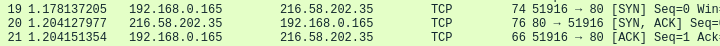
\includegraphics[scale=.65]{Networking Refresher.ThreeWayHandshake.png} 
In this example we can see the three way handshake between the port 51916 from the computer on 192.168.0.165 and the port 80 from the server on 216.58.202.35.

\section{UDP}
UDP stands for User Datagram Protocol and that is a connection-less protocol. This one is used for example in streaming services, DNS, Voice over IP.

\section{Common Ports and Protocols}

\begin{multicols}{2}
\begin{itemize}
\item \textbf{TCP}
\begin{itemize}
\item \textbf{FTP (21)}: File transfer protocol. You can log in and put a file or get a file off the server.
\item \textbf{SSH (22)}: Log into a machine remotely (encrypted).
\item \textbf{Telnet (23)}: Log into a machine remotely (plain text).
\item \textbf{SMTP (25)}: Mail.
\item \textbf{DNS (53)}: Domain Name System: Resolve IP addresses to names.
\item \textbf{HTTP (80) / HTTPS(443)}: Web sites.
\item \textbf{POP3 (110)}: Mail.
\item \textbf{SMB (139 + 445)}: The most common port for pentesters. File shares: think about all the crazy exploits: Wannacry, Eternal Blue, MS17.0.1.0. SMB is open so frequently on networks.
\item \textbf{IMAP (143)}: Mail
\end{itemize}
\end{itemize}

\vfill\null
\columnbreak
\begin{itemize}
\item \textbf{UDP}
\begin{itemize}
\item \textbf{DNS (53)}: Domain Name System: Resolve IP addresses to names.
\item \textbf{DHCP (67, 68)}: Associates you with an IP address, kinda random (from a range). The opposite is static IP address.
\item \textbf{TFTP (69)}: Trivial FTP.
\item \textbf{SNMP (161)}: Simple Network Management Protocol. When we encounter it there may be information to be gathered. Especially if there are strings being used that are public.
\end{itemize}
\end{itemize}

\end{multicols}








\end{document}